\documentclass[submit]{harvardml}

% FDV: Update front matter -- years, dates, references to book sections, etc.
\course{CS181-S22}
\assignment{Assignment \#5}
\duedate{11:59pm EST, April 8, 2021}

\newcommand{\attr}[1]{\textsf{#1}}
\usepackage[OT1]{fontenc}
\usepackage[colorlinks,citecolor=blue,urlcolor=blue]{hyperref}
\usepackage[pdftex]{graphicx}
\usepackage{subfig}
\usepackage{framed}
\usepackage{fullpage}
\usepackage{amsmath}
\usepackage{amssymb}
\usepackage{color}
\usepackage{todonotes}
\usepackage{listings}
\usepackage{common}
\usepackage{bm}
\usepackage{enumitem}
\usepackage{tikz}
\usetikzlibrary{positioning,shapes,arrows}
\usepackage{xifthen}
\usepackage{pythonhighlight}
\usepackage{soul}

\usepackage[mmddyyyy,hhmmss]{datetime}

\definecolor{verbgray}{gray}{0.9}

\lstnewenvironment{csv}{
  \lstset{backgroundcolor=\color{verbgray},
  frame=single,
  framerule=0pt,
  basicstyle=\ttfamily,
  columns=fullflexible}}{}

\begin{document}


\begin{center}
{\Large Homework 5: EM with Mixtures, PCA, and Graphical Models}\\
\end{center}

This homework assignment will have you work with EM for mixtures, PCA,
and graphical models. We encourage you to read sections 9.4 and 8.2.5 of the course textbook.

Please type your solutions after the corresponding problems using this
\LaTeX\ template, and start each problem on a new page.

Please submit the \textbf{writeup PDF to the Gradescope assignment `HW5'}. Remember to assign pages for each question.

Please submit your \textbf{\LaTeX\ file and code files to the Gradescope assignment `HW5 - Supplemental'}. 


\newpage
\begin{problem}[Expectation-Maximization for Gamma Mixture Models, 25pts]

In this problem we will explore expectation-maximization for a Categorical-Gamma Mixture model.

Let us suppose the following generative story for an observation $x$: first one of $K$ classes is randomly selected, and then the features $x$ are sampled according to this class. If $$z \sim \operatorname{Categorical}(\btheta)$$ indicates the selected class, then $x$ is sampled according to the class or ``component'' distribution corresponding to $z$. (Here, $\btheta$ is the mixing proportion over the $K$ components: $\sum_k \theta_k = 1$ and $ \theta_k > 0$). In this problem, we assume these component distributions are gamma distributions with shared shape parameter but different rate parameters: $$x | z \sim \operatorname{Gamma}(\alpha, \beta_k).$$

In an unsupervised setting, we are only given a set of observables as our training dataset: $\mathcal D = \{x_n\}_{n=1}^N$. The EM algorithm allows us to learn the underlying generative process (the parameters $\btheta$ and $\{\beta_k\}$) despite not having the latent variables $\{z_n\}$ corresponding to our training data.

\vspace{2em}

\begin{enumerate}

  \item \textbf{Intractability of the Data Likelihood} We are
    generally interested in finding a set of parameters $\beta_k$ that
    maximizes the likelihood of the observed data: $$\log
    p(\{x_n\}^N_{n=1}; \btheta, \{\beta_k\}^K_{k = 1}).$$ Expand the data
    likelihood to include the necessary sums over observations
    $x_n$ and to marginalize out the latents
    $\boldz_n$. Why is optimizing this likelihood directly
    intractable?

\item \textbf{Complete Data Log Likelihood} The complete dataset
  $\mathcal D = \{(x_n, \boldz_n)\}_{n=1}^N$ includes latents $\boldz_n$. Write
  out the negative complete data log likelihood: $$\mcL(\btheta, \{\beta_k\}^K_{k=1}) =  -\log p(\mathcal D; \btheta, \{\beta_k\}^K_{k=1}).$$

  Apply the power trick and simplify your expression using indicator elements $z_{n
  k}$.\footnote{The ``power trick'' is used when terms in a PDF are raised to the power of indicator components of a one-hot vector.  For example, it allows us to rewrite $p(\boldz_n ;  \btheta) = \prod_k \theta_k^{z_{nk}}$.} Notice that optimizing this loss is now computationally tractable if we know $\boldz_n$.

  (Continued on next page.)

\end{enumerate}

\end{problem}

\newpage


\begin{framed}
\noindent\textbf{Problem 1} (cont.)\\
\begin{enumerate}
\item[3.] \textbf{Expectation Step} Our next step is to introduce a
  mathematical expression for $\boldq_n$, the posterior over the
  hidden component variables~$\boldz_n$ conditioned on the observed data
  $x_n$ with fixed parameters.
That is:
  \begin{align*}
    \textbf{q}_n &= \begin{bmatrix}
      p(\boldz_n =\boldC_1| x_n; \btheta, \{ \beta_k \}^K_{k=1}) \\
      \vdots \\
      p(\boldz_n =\boldC_K| x_n; \btheta, \{ \beta_k \}^K_{k=1})
    \end{bmatrix}.
  \end{align*}
  %
%
  Write down and simplify the expression for
  $\boldq_n$.  Note that because the $\boldq_n$ represents the
  posterior over the hidden categorical variables $\boldz_n$, the
  components of vector $\boldq_n$ must sum to 1.
  The main work is to find an expression for $p(\boldz_n|x_n; \btheta, \{\beta_k\}^K_{k=1})$  for any choice of $\boldz_n$; i.e., for any 1-hot encoded $\boldz_n$. With this, you can then construct the different components that make up the vector $\boldq_n$.
  
\item[4.] \textbf{Maximization Step}
Using the~$\boldq_n$ estimates from the Expectation Step, derive an update for maximizing the expected complete data log likelihood in terms of $\btheta$ and $\{ \beta_k \}^K_{k=1}$.

\begin{enumerate}
    \item Derive an expression for the expected complete data log likelihood using $\boldq_n$.
    \item Find an expression for $\btheta$ that maximizes this expected complete data log likelihood. You may find it helpful to use Lagrange multipliers in order to enforce the constraint $\sum \theta_k = 1$. Why does this optimal $\btheta$ make intuitive sense?
    \item Find an expression for $\beta_k$ that maximizes the expected complete data log likelihood.  Why does this optimal $\beta_k$  make intuitive sense?
\end{enumerate}
    
\item[5.] Suppose that this had been a classification problem. That is,
  you were provided the ``true'' components $\boldz_n$ for each
  observation $x_n$,
  and you were going to perform the classification by
  inverting the provided generative model (i.e. now you're predicting $\boldz_n$ given $x_n$). Could you reuse any of
  your derivations above to estimate the parameters of the model?
  

\item[6.] Finally, implement your solution in \texttt{p1.ipynb} and attach the final plot below.

{\bfseries You will recieve no points for code not included below.}
\end{enumerate}
  
\end{framed}

\newpage
\subsection*{Solution}

\begin{enumerate}
  \item $$ \sum^N_{n=1}log[\sum^k_{k=1}P(x_n,\theta,\beta_k)]$$, unfortunately there is a summation over k inside the log term, which makes this impossible to solve. 9.1 in textbook has more details. 
  \item $$\sum^N_{n=1}\sum^K_{k=1}z_{nk}log(\frac{\beta^\alpha_k}{\Gamma(\alpha)}x^{\alpha-1}e^{-\beta_kx_n} * \prod_k \theta_k^{z_nk})$$
  This is solvable, but only if we know Z. We can get this expression since our expected complete log likeliehood can be defined as $$\sum^N_{n=1}log(p(x_n|z_n;\beta_k)p(z_n|\theta))$$ then we plug in our gamma pdf and use power trick to obtain our answer, yay!
  \item we know that each entry in qn is proportional to $P(x_n|z_n=C_k,\beta_k)*P(z_n=C_k|\theta)$ for class k, and we can plug in gamma pdf times power trick and then normalize to get that index k is  $$\frac{gamma(x_n,\beta_k,\alpha) * \prod_k\theta_k^{z_{nk}}}{\sum_k gamma(x_n,\beta_k,\alpha) * \prod_k\theta_k^{z_{nk}} }$$ Where gamma means the gamma pdf for the probability that $x_n = C_k$, aka we plug $\beta_k, \alpha, x_n$ into gamma pdf  
  \item 
    \begin{enumerate}
      \item $$\sum^N_{n=1}\sum^K_{k=1}q_{nk}ln(\prod_k\theta_k^{C_k}) + q_{nk}ln(gamma(x_n,\alpha,\beta_k))$$ Where "gamma" has the same definition from q3. This is derived through the same process used in 2.1 of the section notes, only we plug in for our probabilities at the end. (write out complete data log likelyhood,then take expected value). 
      \item Take derivative of previous expression plus $-\lambda(\sum_k\theta_k-1)$, our lagrange term and set equal to zero. Our term with gamma doesn't include $\theta$, so it can be ignored. This leaves a simple derivative, which yields:
      $$\frac{\sum^N_{n=1}q_{nk}}{\lambda} = \theta_k$$
      However, we aren't done yet. Now we need to solve for $\lambda$, and we can easily do so by summing over our obtained equation to incude all thetas, which should sum to 1. Then we get that $\lambda = \sum_k\sum_Nq_{nk} = N$,
      so our answer is 
      $$\frac{\sum^N_{n=1}q_{nk}}{N} = \theta_k$$
      This makes inuitive sense because Z is sampled by a categorical of theta, so of course the best value for $\theta_k$ would be the average of the probabilities over the data that $z_n$ is equal to that class. 
      \item 
      Now we take derivative with respect to $\beta_k$ with the lagrange term and set to zero. 
      Fortunately, the only term that has a beta in it is the gamma term, so we write out gamma pdf remove the other terms and take derivative to get $$\sum_Nq_{nk}(\frac{\alpha}{\beta} - x_n) = 0$$
      Then we can simplify to get 
      $$\frac{\alpha\sum_Nq_{nk}}{\sum_Nq_{nk}x_n} = \beta_k$$
      
      Beta is indicates how much the distribution leans leftward from alpha. As beta gets larger than alpha, the distribution leans left and when its smaller it leans right. Summing over the probabilities for $z_n$ and multiplying by alpha and then dividing by the same sum but each weighted by their respective data point gives us how much the distribution for modeling $x|z$ shifts in relation to alpha. 
      
      
    \end{enumerate}
  \item 
  We want a distribution for $Z|X$, We can reuse our generative model to estimate beta, allowing us to form distributions on $x|z$. In turn, we can do $P(z) * P(x|z)$ (we have p(z) now thanks to z being given), to get something proportional to the probability $z|x$, and then normalize that between 0 and 1 by calculating the probabilities for $x|z$ for all classes, and dividing by that number.
  \item 
    Plot:

    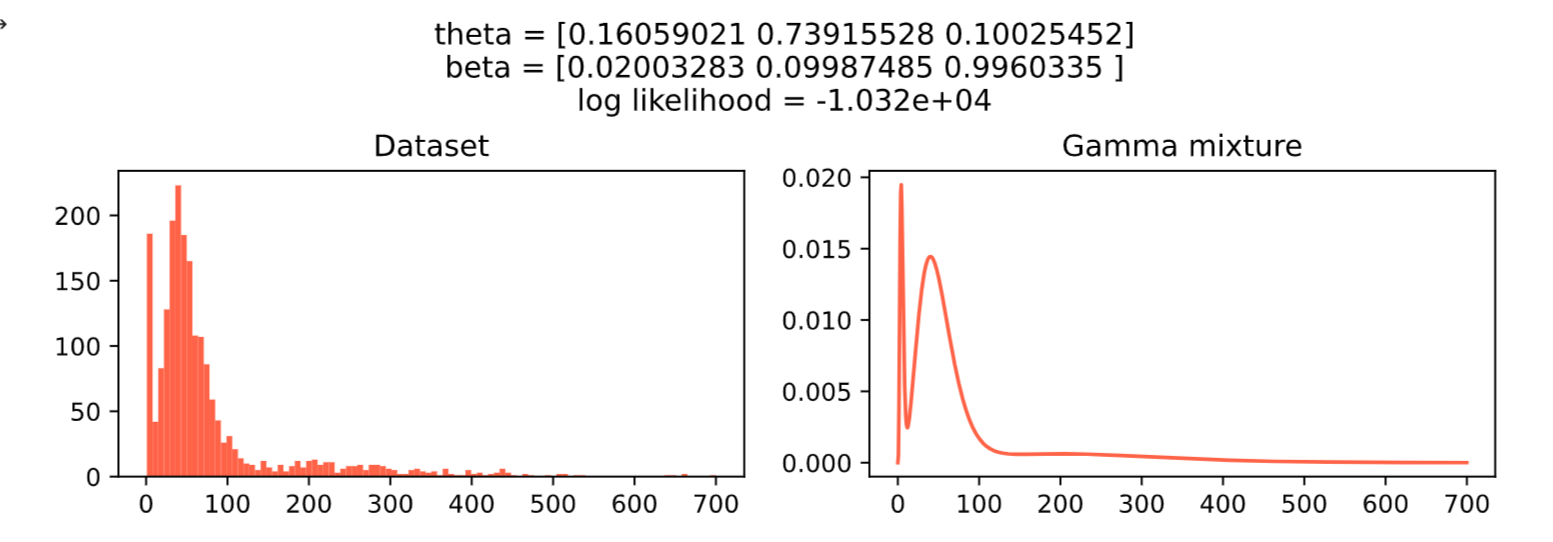
\includegraphics[width=\linewidth]{HW5/Screenshot (162).png}

    Code:

    \begin{python}
def e_step(theta, betas):
    
    proportional = gamma.logpdf(x,alpha, scale=1/betas) + np.log(theta)
 
        
    q = np.subtract(proportional,logsumexp(proportional,axis=1, keepdims=True))


    return (np.exp(q))


def m_step(q):

    
    theta_hat = q.sum(0) / len(q)
    beta_hats = (q.sum(0) * alpha) / (q*x).sum(0)
    
    return theta_hat, beta_hats


def log_px(x, theta, betas):
    p = gamma.logpdf(x,alpha,scale=1/betas) + np.log(theta)
    return logsumexp(p,axis=1)


def run_em(theta, betas, iterations=1000):
    while iterations > 0:
      q = e_step(theta, betas)
      theta,betas = m_step(q)
      iterations = iterations -1 
    return theta, betas
    \end{python}
\end{enumerate}


\newpage

\begin{problem}[PCA, 15 pts]

% FDV: Here are the notes from last year.  I've already edited to make clear we want L2.  As noted below, we should also provide the baseline/reference to the pset 4 solutions in case they computed that wrong somehow.  
% 
% # problem 2 clarifications
% *NB: There was a lot of confusion about this problem, and we ended up accepting any form of comparison to PCA. Next year should clarify which norm students should use more explicitly (and maybe provide a baseline for students if the computation of the reconstruction error is different from what students calculated on pset4.)*
% 
% For Problem 2.3 (computing PCA reconstruction error), we will accept both the L1 and L2 norm and both summing over the errors for individual images and taking the mean of the errors (as long as you compute the error for K-Means the same way as you compute it for PCA). Apologies for the ambiguity in this question! 

  
For this problem you will implement PCA from scratch on the first 6000 images of the MNIST dataset. Your job is to apply PCA on MNIST and discuss what kind of structure is found. Implement your solution in \texttt{p2.ipynb} and attach the final plots below.

{\bfseries You will recieve no points for using third-party PCA implementations (i.e. {\normalfont \texttt{scikit-learn}}).}

{\bfseries You will recieve no points for code not included below.}
\begin{enumerate}

\item Compute the PCA. Plot the eigenvalues corresponding to the most
  significant 500 components in order from most significant to
  least. Make another plot that describes the cumulative proportion of
  variance explained by the first $k$ most significant components for
  values of $k$ from 1 through 500.  How much variance is explained by
  the first 500 components?  Describe how the cumulative proportion of
  variance explained changes with $k$.  Include this plot below.

\item Plot the mean image of the dataset and plot an image
  corresponding to each of the first 10 principle components.  How do
  the principle component images compare to the cluster centers from
  K-means? Discuss any similarities and differences.  Include these
  two plots below.

  \textit{Reminder: Center the data before performing PCA}

\item Compute the reconstruction error on the data set using the mean
  image of the dataset.  Then compute the reconstruction error using
  the first 10 principal components.  How do these errors compare to
  the final objective loss achieved by using K-means on the dataset?
  Discuss any similarities and differences.

  For consistency in grading, define the reconstruction error as the squared L2
  norm averaged over all data points.

\item Suppose you took the original matrix of principle components
  that you found $U$ and multiplied it by some rotation matrix $R$.
  Would that change the quality of the reconstruction error in the
  last problem?  The interpretation of the components?  Why or why
  not?
  
\end{enumerate}


\end{problem}

\newpage
\subsection*{Solution}
Plots:

 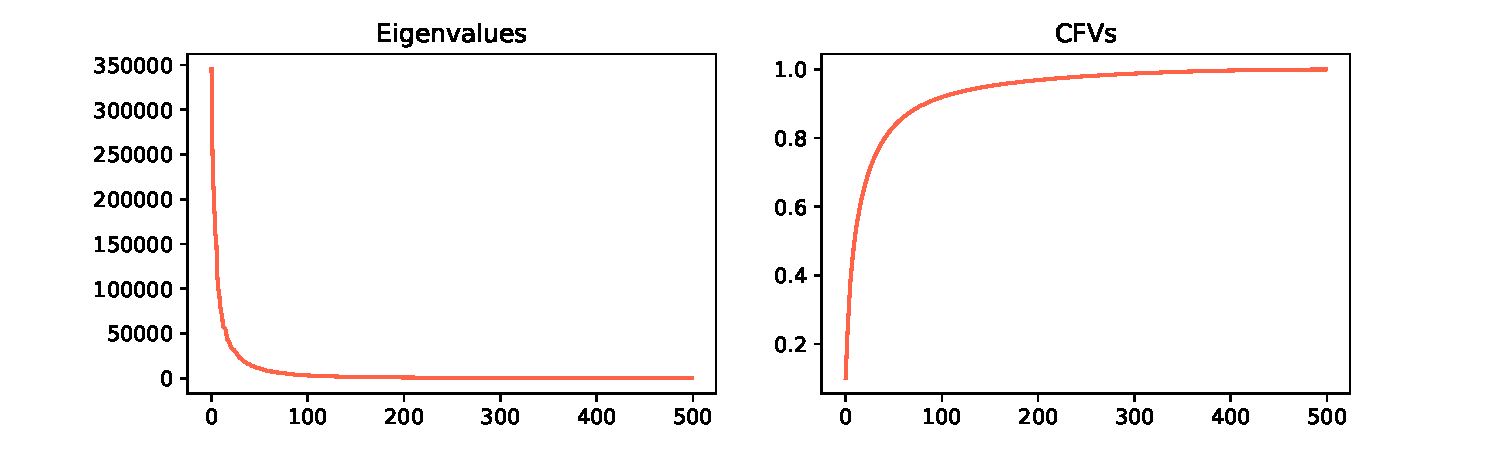
\includegraphics[width=\linewidth]{HW5/p2_cfvs (6).pdf}


\includegraphics[width=0.25\linewidth]{p2_mean}
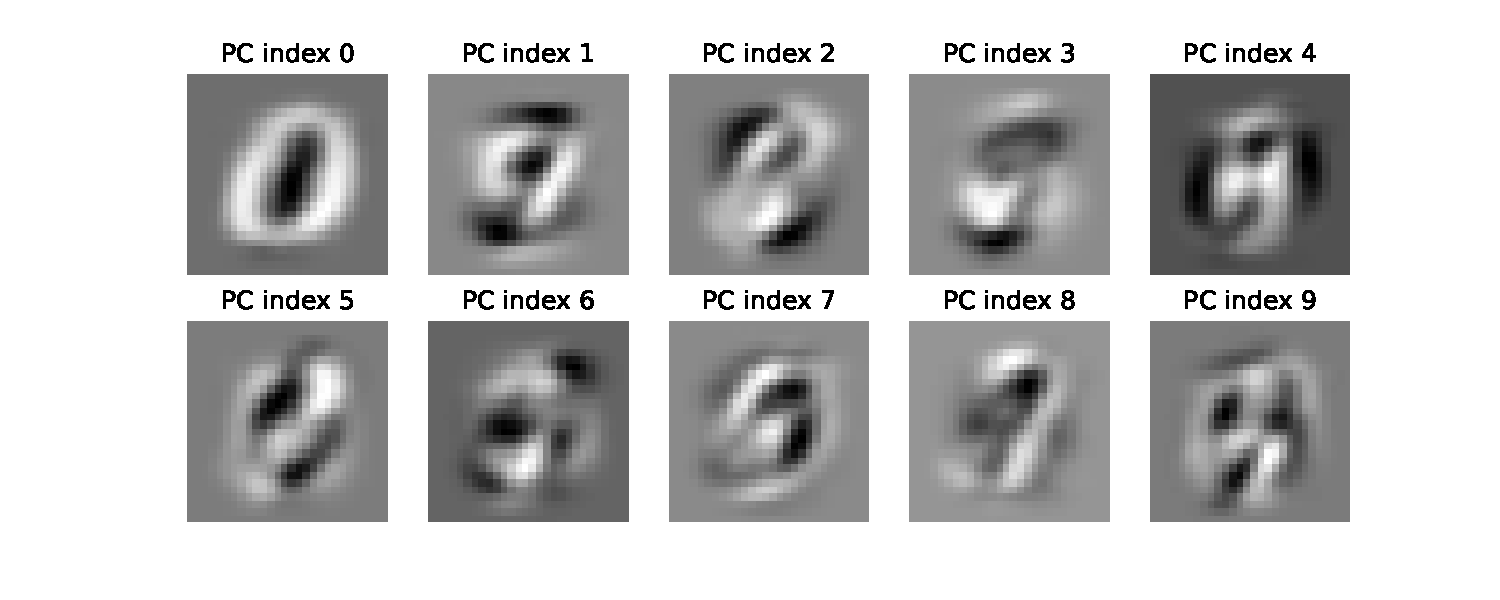
\includegraphics[width=0.75\linewidth]{p2_pcomps}



\begin{python}
from re import X
def pca(x, n_comps=500):
    
    xmean = np.mean(x,axis=0)
    x = np.subtract(x,xmean) #subtract mean from datapoints
    cov = x.T@x/N # find covariance matrix
    u,sig,v = np.linalg.svd(cov)
    top_eigvals = sig[:n_comps] #no need to square, since np.linalg.svd does cov@cov.t or cov.T@cov first
    top_pcomps = v[:n_comps] 



    return top_eigvals, top_pcomps


def calc_cfvs(eigvals):
    cum_frac_vars = np.cumsum(eigvals)/np.sum(eigvals)
    return cum_frac_vars


def calc_errs(x, pcomps):
    x_mean = np.array([np.mean(x,axis=0)])
    xmean = x - x_mean
    err_mean = (np.linalg.norm(x-x_mean))**2/6000
    reduced = pcomps@xmean.T # calculating time series, decomposing dataset into principal components
    reconst = pcomps.T@reduced # reconstructing dataset
    recontmean = reconst + x_mean.T #transposes for getting around stupid broadcasting reqs


    err_pcomp = ((np.linalg.norm(x-recontmean.T, axis=1))**2).mean()


    return err_mean, err_pcomp
\end{python}

\begin{enumerate}
  \item As K increases, the variance explained increases very rapidly at first and then slows down, getting closer and closer to 1 over time. Meanwhile, the eigenvalues graph is the opposite of this which makes sense since each eigenvalue is variance from that eigenvector. 
  
  \item The principal components look similar to the standardized kmeans plots as they kinda have the white circles at the edges of the principal components. 
  although these ones don't really represent numbers like the kmeans clusteroids did. While u may be able to make out 1 or 2 numbers, the principal components are really just common ways in which the pixels may be arrayed so that we can reconstruct the data the best with that vector. While kmeans foccuses on good clusters, here we are fousing on storing data with orthogonal vectors. 
  
  \item Reconstruction error (using mean): 3.435796e+06
Reconstruction error (using mean and top 10 pcomps): 1.731315e+06
Final objective loss: estimating based on graph from last pset, error was approx 7e8, and need to divide that by number of datapoints which was 300, which yields an error of approx 2.333e+06, which is much higher than PCA but lower than using mean, which makes sense since mean is just using kmeans with k = 1. However, while kmeans may have better served for giving us clusters that represnt actual numbers, PCA seems to have much lower loss. This makes sense given that PCA is a method that minimizes reconstruction loss by projecting to orthogonal axises optimally, rather than finding good clusters. 

  \item Rotating the principal components would change the basis to which we are projecting, and would decrease the amount of variance explained by the first few components which is what we are maximizing with PCA.This could increase Reconstruction error, however, the rotation can be used to see how much components vary along a specific axis, which is helpful for interpreting specifics when one has prior knowledge about the dataset. 
Code:
\end{enumerate}

\newpage

\begin{problem}[Bayesian Networks, 10 pts]

% FDV: I think we can keep this problem as-is, and just clarfiy based
% on notes from last year.
% # problem 3 clarifications
% The phrasing of Q3 is slightly off because it implies that you need to explain why each path is not blocked in the case that two nodes are not independent. It is sufficient to provide a single unblocked path. Better phrasing is (emphasis added) "Use the concept of d-separation to answer the questions and show your work (i.e., state what the blocking path(s) is/are and which node blocks the path; or explain why there exists a path that is not blocked)." 
% 
% Some helpful resources for d-separation:  The 2020 Section 8 notes, Bishop p. 372 - 379, Section 8.2 of the CS 181 textbook
% 
% Problem 3: Make it clear (put the instructions in one place) that we require explanations for both "yes" and "no" answers

  
  \noindent In this problem we explore the conditional independence
  properties of a Bayesian Network.  Consider the following Bayesian
  network representing a fictitious person's activities. Each random
  variable is binary (true/false).

\begin{center}
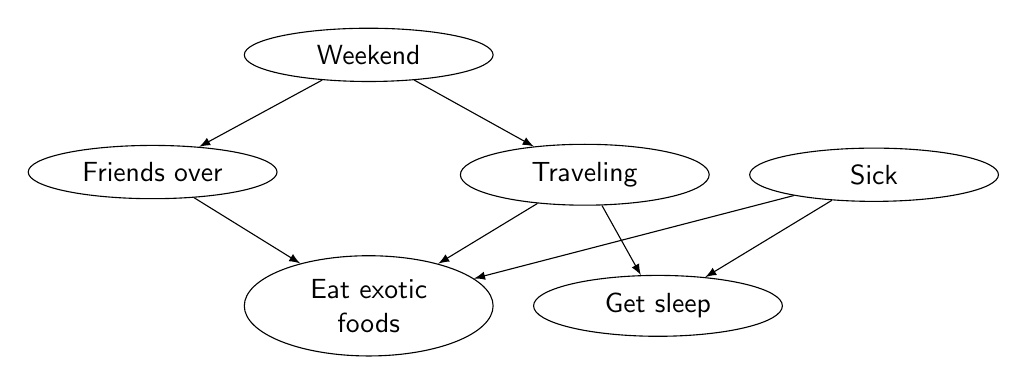
\begin{tikzpicture}[
  node distance=1cm and .5cm,
  bn/.style={draw,ellipse,text width=2cm,align=center}
    ]
    \node[bn] (w) {\attr{Weekend}};
    \node[bn,below right=of w] (t) {\attr{Traveling}};
    \node[bn,right=of t] (s) {\attr{Sick}};
    \node[bn,below left=of w] (f) {\attr{Friends over}};
    \node[bn,below right=of f] (eef) {\attr{Eat exotic foods}};
    \node[bn,right=of eef] (gs) {\attr{Get sleep}};
    \path (w) edge[-latex] (t)
    (w) edge[-latex] (f)
    (f) edge[-latex] (eef)
    (t) edge[-latex] (eef)
    (t) edge[-latex] (gs)
    (s) edge[-latex] (gs)
    (s) edge[-latex] (eef);
    \end{tikzpicture}
\end{center}

The random variables are:

\begin{itemize}
\item \attr{Weekend}: Is it the weekend?
\item \attr{Friends over}: Does the person have friends over?
\item \attr{Traveling}: Is the person traveling?
\item \attr{Sick}: Is the person sick?
\item \attr{Eat exotic foods}: Is the person eating exotic foods?
\item \attr{Get Sleep}: Is the person getting sleep?
\end{itemize}

\medskip

For the following questions, $A \perp B$ means that events A and B are
independent and $A \perp B | C$ means that events A and B are independent
conditioned on C.

\textbf{Use the concept of d-separation} to answer the
questions and show your work (i.e., state what the blocking path(s) is/are and what nodes block the path; or explain why each path is not blocked).

\textit{Example Question:} Is $\attr{Friends over} \perp \attr{Traveling}$? If NO, give intuition for why.

\textit{Example Answer:} NO. The path from Friends over -- Weekend -- Traveling is not blocked following the d-separation rules as we do not observe Weekend. Thus, the two are not independent. 

\textbf{Actual Questions:}

\begin{enumerate}
\item Is $\attr{Weekend} \perp \attr{Get Sleep}$?
  If NO, give intuition for why.

\item Is $\attr{Sick} \perp \attr{Weekend}$?
  If NO, give intuition for why.


\item Is $\attr{Sick} \perp \attr{Friends over}\given \attr{Eat exotic
  foods}$? If NO, give intuition for why.


\item Is $\attr{Friends over} \perp \attr{Get Sleep}$? If NO, give
  intuition for why.

\item Is $\attr{Friends over} \perp \attr{Get Sleep} \given
  \attr{Traveling}$? If NO, give intuition for why.

\item Suppose the person stops traveling in ways that affect their
  sleep patterns.  Travel still
  affects whether they eat exotic foods.  Draw the modified network. (Feel free to reference the handout file for the commands for displaying the new network in \LaTeX).

\item For this modified network, is $\attr{Friends over} \perp
  \attr{Get Sleep}$? If NO, give an intuition why.  If YES,
  describe what observations (if any) would cause them to no longer be
  independent.

\end{enumerate}
\end{problem}

\newpage
\section*{Solution}
\begin{enumerate}
  \item No, since weekend gives us information about traveling, which gives us information about getting sleep.
  \item Yes
  \item No, since we know exotic foods. (If friends over mean high chance of exotic food but it doesnt happen and sick means low chance of exotic food, and we know he ate exotic food, then knowing he was sick indicates high chance friends over because sick and then eat exotic food unlikely)
  \item No, friends over is connected via weekend - traveling - get sleep
  \item yes
  \item \begin{center}
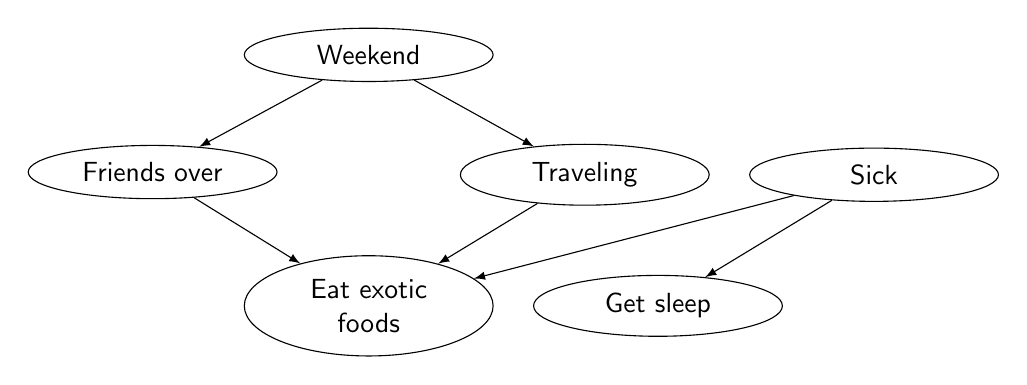
\begin{tikzpicture}[
  node distance=1cm and .5cm,
  bn/.style={draw,ellipse,text width=2cm,align=center}
    ]
    \node[bn] (w) {\attr{Weekend}};
    \node[bn,below right=of w] (t) {\attr{Traveling}};
    \node[bn,right=of t] (s) {\attr{Sick}};
    \node[bn,below left=of w] (f) {\attr{Friends over}};
    \node[bn,below right=of f] (eef) {\attr{Eat exotic foods}};
    \node[bn,right=of eef] (gs) {\attr{Get sleep}};
    \path (w) edge[-latex] (t)
    (w) edge[-latex] (f)
    (f) edge[-latex] (eef)
    (t) edge[-latex] (eef)
    (s) edge[-latex] (gs)
    (s) edge[-latex] (eef);
    \end{tikzpicture}
\end{center}
  \item 
  yes, however, observing eat exotic foods can change this. Eat exotic foods is unobserved, so it blocks information flow to get sleep under d seperation rules.  Because if no friends over, traveling/sick informs exotic food, so we get a bit of information about those two, which gives us a bit of information about get sleep. 
\end{enumerate}

\newpage
%%%%%%%%%%%%%%%%%%%%%%%%%%%%%%%%%%%%%%%%%%%%%
% Name and Calibration
%%%%%%%%%%%%%%%%%%%%%%%%%%%%%%%%%%%%%%%%%%%%%
\subsection*{Name}
Johan Vlassak

\subsection*{Collaborators and Resources}
Whom did you work with, and did you use any resources beyond cs181-textbook and your notes?
I worked with a few people at office hours and np documentation. I worked with Kidist and Luke aswell. 
\subsection*{Calibration}
Approximately how long did this homework take you to complete (in hours)? 
15
\end{document}
